\subsection{Chapter 20 - Magnetic force}

\subsubsection{Overview}\label{chapter:magneticforce}

This chapter introduces the tools to model the magnetic force, which is something that we have all experienced with magnets. As we will see, the magnetic force acts on moving (electric) charges, and is thus fundamentally different from the electric force which acts on stationary and moving charges. In later chapters, we will develop the tools that allow us to make connections between the electric and magnetic fields.

\begin{framed}
\textbf{Learning Objectives}\\
\begin{itemize}
\item Understand the key characteristics of a magnetic field and what makes it different from an electric field.
\item Understand how to model the magnetic force on a moving charge.
\item Understand how to model the magnetic force on a wire carrying current.
\item Understand how to model the torque exerted on a current-carrying loop by a magnetic field.
\item Understand how to model the Hall Effect.
\item Understand simple applications of the magnetic force.
\end{itemize}
\end{framed}

\begin{framed}
\textbf{Think About It}\\
When you go through airport security, they sometimes sample your luggage with sticky tape and place that tape into a machine to detect trace amounts of explosives. How does that machine work?

\begin{enumerate}
\item The machine detects trace amounts by ``sniffing'' the sample using similar chemical reactions as those in our olfactory system.
\item The machine vaporizes the sample and accelerates the resulting charged vapour around a circle to determine its constituents.
\end{enumerate}

\begin{framed}
\textbf{Answer}\\
\begin{enumerate}[resume]
\item
\end{enumerate}
\end{framed}
\end{framed}

\subsubsection{Magnetic fields}

Just as we can model the electric force on a charge by using the electric field (e.g. from another charge), we can model the force on a magnet by using a magnetic field (e.g. from another magnet). In your experience, every magnet that you have seen always has a ``North'' pole and a ``South'' pole. Most likely, you have noticed that the North pole of a magnet is attracted to the South pole of another magnet, and that the two North (or South) poles of different magnets repel each other. Thus, the magnetic force is attractive between two opposite poles, and repulsive otherwise.

The Earth itself can be modelled as a giant bar magnet, with North and South magnetic poles. The poles on a magnet are labelled North and South according to which geographic pole of the Earth they are attracted to (a magnetic compass needle has a magnetic North pole on the side that point to the Earth's North geographic pole).

\begin{framed}
\textbf{Checkpoint}\\
Is the magnetic North pole of the Earth located closer to the Earth's geographic North pole or closer to its geographic South Pole?

\begin{enumerate}
\item Earth does not have a magnetic field.
\item Earth's magnetic North pole is at Earth's geographic North pole.
\item Earth's magnetic North pole is at Earth's geographic South pole.
\item Earth's magnetic North pole depends on the charge of the observer.
\end{enumerate}

\begin{framed}
\textbf{Answer}\\
\begin{enumerate}[resume]
\item
\end{enumerate}
\end{framed}
\end{framed}

It may seem that the magnetic force can be described in the same way as the electric force, having two opposite sign ``charges'' (or poles for magnets), although this is not the case. As far as we can tell, there are no magnets that have only a North or a South pole. Every magnet must have a North \textit{and} a South pole. This is fundamentally different from the electric force, where an object can have a net positive or negative charge. In the context of magnetism, we say that ``monopoles do not exist'' (an object that has only a North or a South pole would be called a monopole). This is illustrated in Figure~\ref{fig:magneticforce:magnetcut}, which shows what happens as one cuts a bar magnet into two pieces; rather than ending up with a North and a South piece (monopoles), we end up with two smaller bar magnets, each with their own North and South pole.

\begin{figure}[!htbp]
\centering
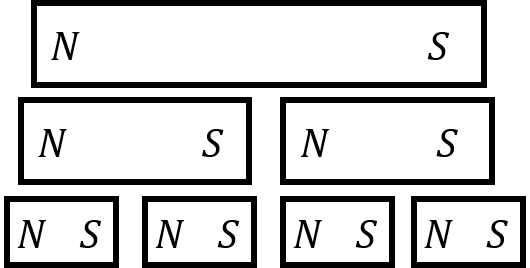
\includegraphics[width=0.4\linewidth]{files/magnetcut-3c8cc38e7c5df139fbe1d25b9b3412a6.png}
\caption[]{When a bar magnet is cut through the middle, one obtains two magnets, each with a North and South pole, rather than a North and a South magnet.}
\label{fig:magneticforce:magnetcut}
\end{figure}

We model the magnetic force using a magnetic field vector, usually labelled $\vec B$. The magnitude of the magnetic field has the S.I. units of Teslas ({\textbackslash}si\{T\}). We draw magnetic field lines in much the same way that we draw electric field lines. The magnetic field lines are such that the magnetic field vector, $\vec B$, at some point in space is tangent to the field line at that point. The strength of the magnetic field is determined by the density of field lines at that position in space. The direction of the magnetic field, $\vec B$, indicates the direction of the force that is exerted on the North pole of a magnet. Magnetic field lines thus flow away from North poles and towards South poles.

The magnetic field description is similar to that of the electric field, with North magnetic poles being similar to positive electric charges, and vice versa.  However, because magnetic monopoles do not exist, magnetic field lines do not end (or start) on the pole of a magnet. Rather, magnetic field lines must always form \textbf{closed loops}. Figure~\ref{fig:magneticforce:barfield} shows the magnetic field lines for a bar magnet, highlighting that the field lines do not end at the poles, but rather continue through the magnet (and some of the lines only ``close'' outside of the figure). The magnetic field from a bar magnet is very similar to the electric field created by an electric dipole. For that reason, an object (such as a bar magnet) that forms magnetic field lines of this shape are often described as magnetic dipoles.

\begin{figure}[!htbp]
\centering
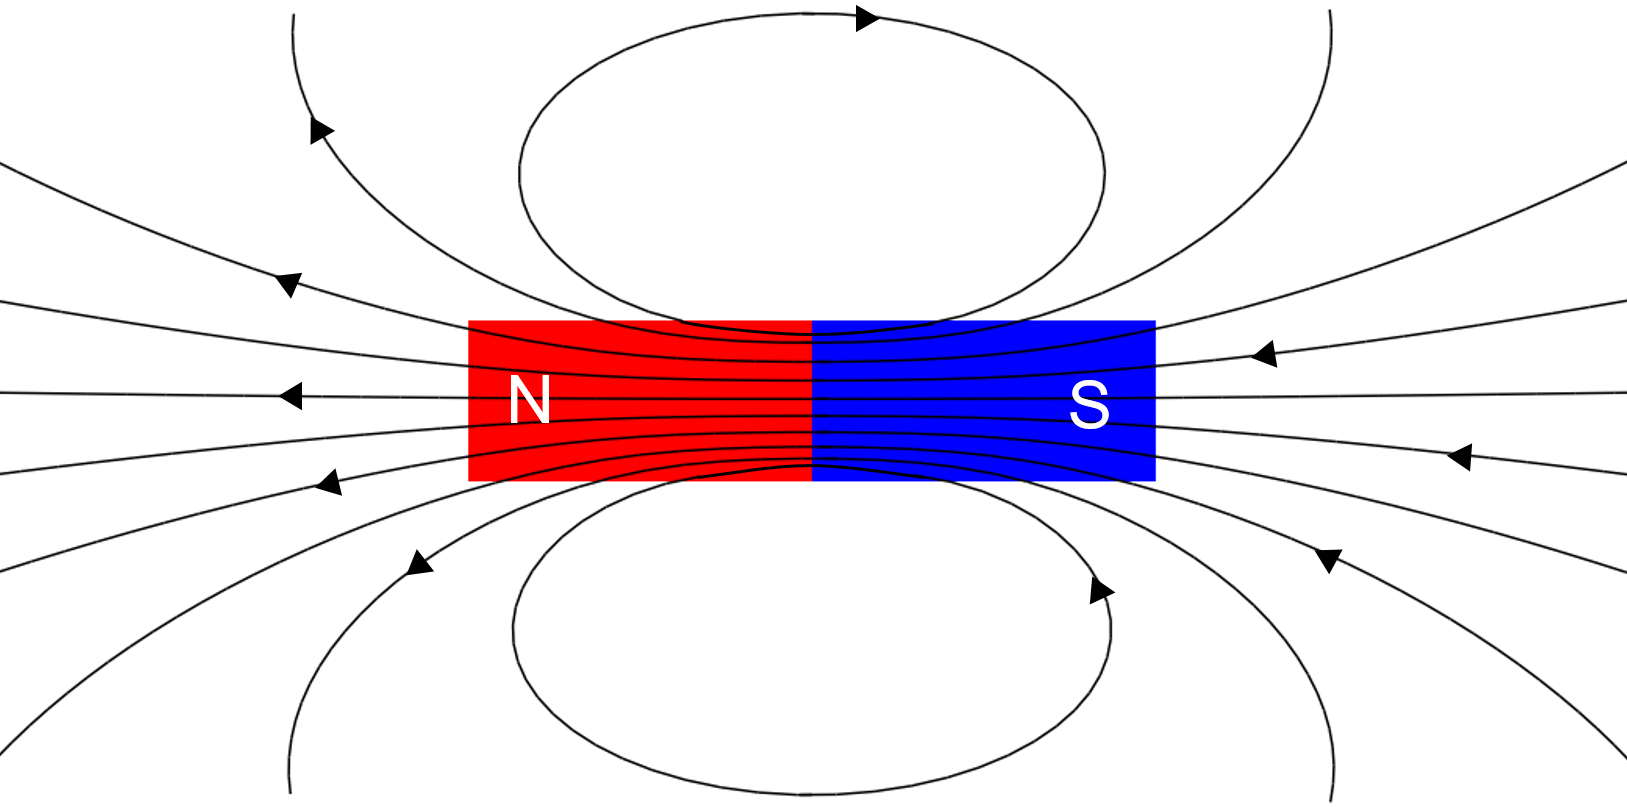
\includegraphics[width=0.55\linewidth]{files/barfield-6229f75cb4409fdf87afdb0d239dbb7e.png}
\caption[]{The magnetic field lines for a bar magnet always form closed loops as they do not end at the North or South pole of the magnet.}
\label{fig:magneticforce:barfield}
\end{figure}

We will discuss how to model magnetic fields in the next chapter, but it is important to understand that magnetic fields are created by moving electric charges. The electrons in the material that forms a bar magnet are the moving charges that create the magnetic field. As we will see, the magnetic field from a charge moving around in a circle (or a circular loop of current), has exactly the same shape as that of a bar magnet, as illustrated in Figure~\ref{fig:magneticforce:loopfield}. We can thus think of charge moving in a circle as a small bar magnet, or more precisely, as a magnetic dipole.

\begin{figure}[!htbp]
\centering
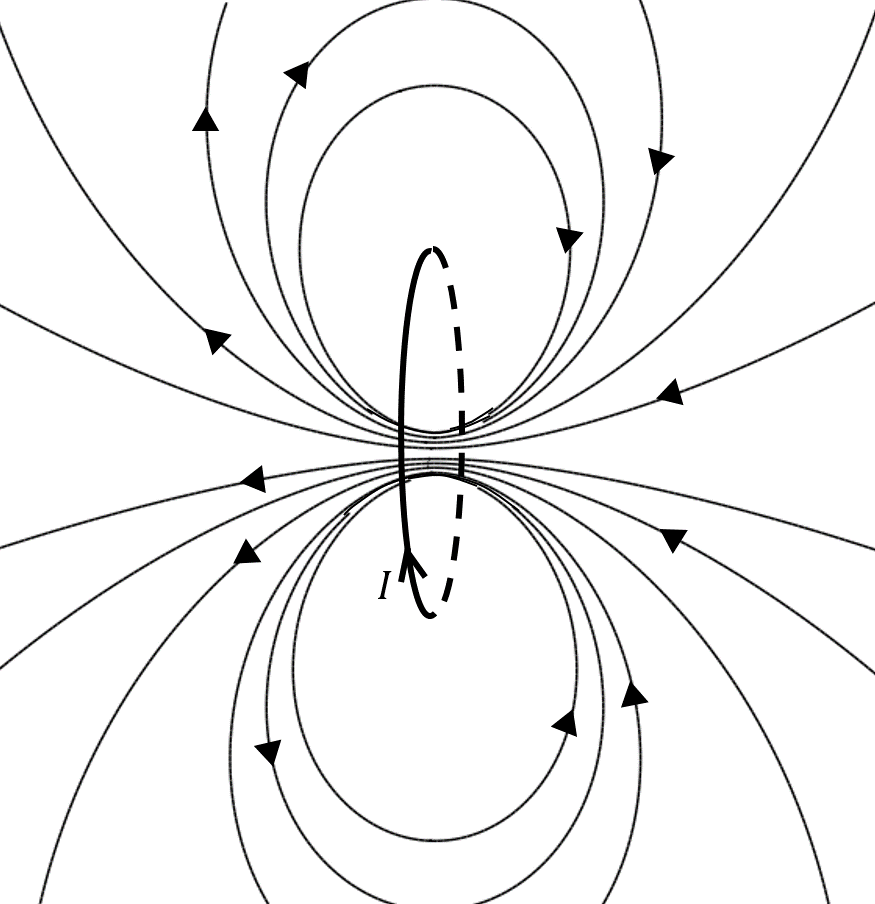
\includegraphics[width=0.45\linewidth]{files/loopfield-c0b99f3b0aaa1c8e1f9f3ca5dc35a9a2.png}
\caption[]{The magnetic field lines produced by a circular loop of current, $I$, are the same as those produced by a bar magnet.}
\label{fig:magneticforce:loopfield}
\end{figure}

In a magnet, the electrons in the material are moving in such a way that the magnetic fields that they generate are all in the same direction. In other words, each atom is like a small magnetic dipole, and all of these are aligned. This allows us to understand why cutting a magnet does not result in two monopoles (Figure~\ref{fig:magneticforce:magnetcut}): when we cut the bar magnet, we end up with less material, but each piece of material still contains magnetic dipoles that are aligned with each other, each having a North and South pole. Note that it is not the motion of electrons around their nuclei that results in the magnetic field, and that one  requires quantum mechanics and the notion of ``spin'' to describe this all in detail.

Most materials will respond to magnetic fields, but the behaviour is most evident in ``ferromagnetic'' materials, such as iron (Fe). Ferromagnetic materials can be magnetized by an external magnetic field, effectively transforming them into magnets. One can think of a material as containing many little magnetic dipoles (from the motion of the electrons), which themselves are like bar magnets. If that material is ferromagnetic,  an external magnetic field can act on the little ``bar magnets'', orienting them all in the same way, so that the material as a whole becomes magnetic. For some ferromagnetic materials, that common orientation will remain when the external magnetic field is removed, creating a ``permanent magnet''. For other ferromagnetic materials, the common orientation disappears when the external field is removed; those materials are thus attracted to a magnet, but they cannot form a magnet.

\subsubsection{The magnetic force on a moving charge}

\begin{framed}
\textbf{Review}\\
Before proceeding, you may wish to review:

\begin{itemize}
\item Section~\ref{sec:Vectors:vectorproduct} on the vector product.
\end{itemize}
\end{framed}

When an electric charge, $q$, has a velocity, $\vec v$, relative to a magnetic field, $\vec B$, a magnetic force is exerted on the particle:
\begin{equation}
\boxed{\vec F_B = q \vec v \times \vec B}
\end{equation}
We can make a few remarks about the magnetic force:

\begin{itemize}
\item The magnetic force is always perpendicular to the velocity and to the magnetic field (since it is given by their cross-product).
\item The direction of the magnetic force depends on the sign of the charge.
\item The magnetic force can do no work, since it is always perpendicular to the velocity (and thus to displacement).
\item There is no force if the particle's velocity is in the same direction as the magnetic field vector.
\item The force increases with charge, speed, and strength of the magnetic field.
\end{itemize}

\begin{framed}
\textbf{Checkpoint}\\
A proton moves East in Earth's magnetic field, which way is it deflected?

\begin{enumerate}
\item Away from the Earth.
\item Towards the Earth.
\item North.
\item South.
\end{enumerate}

\begin{framed}
\textbf{Answer}\\
\begin{enumerate}
\item
\end{enumerate}
\end{framed}
\end{framed}

\begin{framed}
\textbf{Checkpoint}\\
An electron moves West in Earth's magnetic field, which way is it deflected?

\begin{enumerate}
\item Away from the Earth.
\item Towards the Earth.
\item North.
\item South.
\end{enumerate}

\begin{framed}
\textbf{Answer}\\
\begin{enumerate}
\item
\end{enumerate}
\end{framed}
\end{framed}

\begin{framed}
\textbf{Josh's Thoughts}\\
\{\}
It is very important to remember what each part of the right-hand rule for cross-products represents. To help remember what each finger represents, I say ``velocity'' as I extend my thumb, ``field'' as I extend my index finger, and ``force'' as I extend my middle finger. When using the right hand rule, it is also important to remember the $q$ in the equation $\vec F_B = q\vec v \times \vec B$. This $q$ could be negative, which would mean that the force acts in the opposite direction.

\begin{figure}[!htbp]
\centering
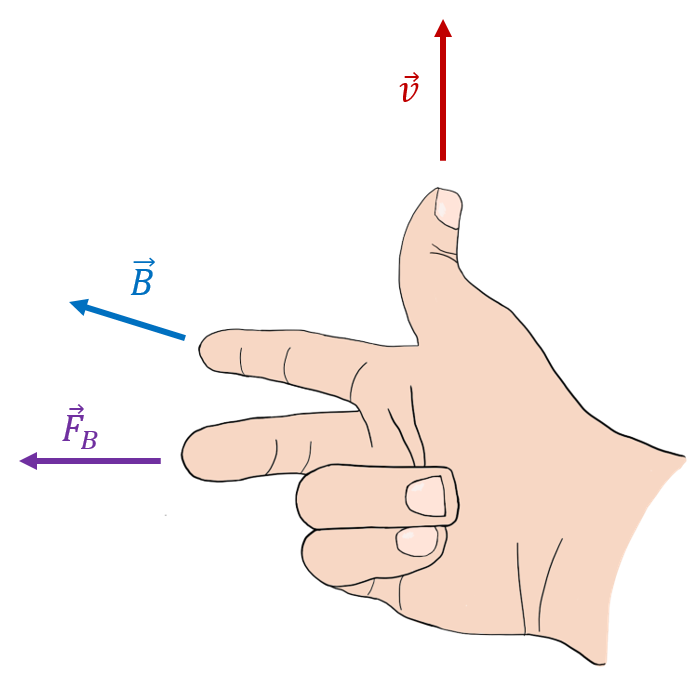
\includegraphics[width=0.4\linewidth]{files/rhr-0a145067c9b8e339abb2d3735e257d33.png}
\caption[]{The way that Josh remembers the right hand rule for magnetism.}
\label{fig:magneticforce:rhr}
\end{figure}

If you find yourself forgetting the right-hand rule on a test or exam, just remember that you can still find the correct answer by setting up a three-dimensional coordinate system and evaluating the cross product.
\end{framed}

You should be somewhat bothered by the fact that the force depends on the velocity of the charge, since velocity depends on the frame of reference from which it is measured. The above equation has a strange implication: if we observe an electron moving in a magnetic field, we will see its motion be deflected by the magnetic field. If we move along with the electron, so that it has a velocity of zero in our frame of reference, we should not see the electron being deflected, since the magnetic force would be zero. Clearly, the motion of the electron cannot depend on the frame of reference from which we observe it. Thus, the only way that this equation can make sense is if the magnetic field also depends on our frame of reference. We will revisit this in a subsequent chapter, but for now, remember that this equation only makes sense if the velocity is measured in the same reference frame as that in which the magnetic field is defined.

Another bothersome issue with the magnetic force is that it appears to depend on the fact that most humans are right-handed. Indeed, the direction of the force requires one to use the right-hand rule, which appears arbitrary. This is a common occurrence in physics, as many quantities are defined using a cross-product. However, no physical quantity can ever depend on our choice of right or left hand for determining cross-products. It turns out that any physical quantity (such as the force on a particle, which will deflect the particle in a clearly identifiable direction that does not depends on a human's choice of right and left), always depends on two successive applications of the right-hand rule. In this case, the direction of the magnetic field is also given by a right-hand rule applied to the moving charges that create the field (as we will see in the next chapter). The successive uses of the right hand twice ``cancel''; one finds that a charge is deflected in the same direction if one had used the left hand to define the magnetic field, and then again the left-hand for the cross-product! We will revisit this issue in the next chapter.

Consider the motion of a charged particle in a region where the magnetic field is uniform (constant in magnitude and direction). If the velocity vector of the particle is perpendicular to the magnetic field, the particle will undergo uniform circular motion, as illustrated in Figure~\ref{fig:magneticforce:cyclotron}.

\begin{figure}[!htbp]
\centering
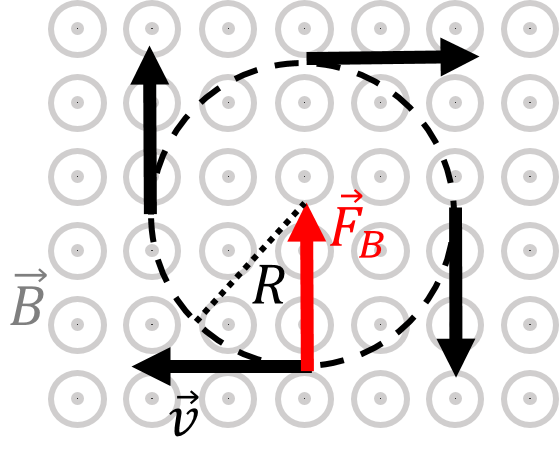
\includegraphics[width=0.35\linewidth]{files/cyclotron-e4bb14fd18f077d23ca915fb07671ad1.png}
\caption[]{The motion of a charged particle in a uniform magnetic field (out of the page) is uniform circular motion.}
\label{fig:magneticforce:cyclotron}
\end{figure}

Indeed, the force is always perpendicular to the velocity, and the force is constant in magnitude since both the speed and magnetic field remain constant. These are the only conditions required for uniform circular motion. We can easily determine the radius, $R$, of the circle, since the magnetic force is responsible for the centripetal acceleration:
\begin{equation}
F_B &= m\frac{v^2}{R}\\
qvB &= m\frac{v^2}{R}\\
\therefore R &= \frac{mv}{qB}
\end{equation}
The radius is called the ``cyclotron radius''.

\begin{framed}
\textbf{Checkpoint}\\
Is the particle illustrated in Figure~\ref{fig:magneticforce:cyclotron} positively or negatively charged?

\begin{enumerate}
\item The particle is positively charged.
\item The particle is negatively charged.
\item Not enough information to tell.
\item The particle has no charge.
\end{enumerate}

\begin{framed}
\textbf{Answer}\\
\begin{enumerate}
\item
\end{enumerate}
\end{framed}
\end{framed}

Referring to Figure~\ref{fig:magneticforce:cyclotron}, if the velocity of the particle is in the plane of the page (perpendicular to the magnetic field), as illustrated, the particle will undergo uniform circular motion. If the velocity of the particle has a component that is parallel to the magnetic field (for example a component coming out of the page, towards you), the particle will undergo ``helical motion'' (a spiral). The radius of the helix is determined by the component of the velocity, $\vec v_{\perp}$, that is perpendicular the magnetic field:
\begin{equation}
\therefore R &= \frac{mv_{\perp}}{qB}
\end{equation}
The charged particle would also have a component of velocity towards you that is constant, resulting in the spiral motion illustrated in Figure~\ref{fig:magneticforce:helix}. Note that the distance between two spirals (labelled $h$ in the figure) is called the ``pitch'', and is determined by the component of velocity that is parallel to the magnetic field, $\vec v_\parallel$, since that component is not affected by the magnetic force.

\begin{figure}[!htbp]
\centering
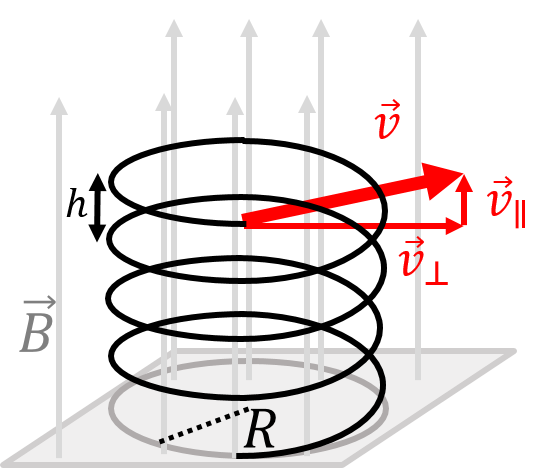
\includegraphics[width=0.4\linewidth]{files/helix-31124e86652b21b8c075857e84aca2d0.png}
\caption[]{The helical motion of a charged particle with a component of velocity parallel to the magnetic field. The distance, $h$, between spirals is called the ``pitch''.}
\label{fig:magneticforce:helix}
\end{figure}

\begin{framed}
\textbf{Example 20.1}\\
A particle of unknown charge and unknown mass is observed to undergo uniform circular motion with a period, $T$, when travelling perpendicular to a uniform magnetic field, $B$. What is the ratio of the particle's charge to its mass, $q/m$?

\begin{framed}
\textbf{Solution}\\
We can use the period of the motion to determine the speed of the particle in terms of the radius of the circular path:
\begin{equation}
v = \frac{2\pi R}{T}
\end{equation}
and then use the equation for the cyclotron radius to relate this to the charge-to-mass ratio of the particle:
\begin{equation}
R &= \frac{mv}{qB}\\
  &= \frac{2\pi R m}{qBT}\\
\therefore \frac{q}{m} &= \frac{2\pi}{BT}
\end{equation}
\textbf{Discussion:} When a charged particle undergoes uniform circular motion in a magnetic field, the radius of the motion depends on the particle's charge-to-mass ratio. This can often be used to measure the mass of, say, an ion, if the charge of the ion is known (usually one or two units of the electron charge). A mass spectrometer makes use of this principle in order to determine the composition of a sample. The sample is vaporized and ionized, the ions are then accelerated using an electric potential difference, before they undergo uniform circular motion. Ions of different masses (and same charge) will then undergo circular motion with different radii, which allows their masses to be determined, and thus the composition of the sample to be known.
\end{framed}
\end{framed}

\subsubsection{The magnetic force on a current-carrying wire}

\begin{framed}
\textbf{Review}\\
Before proceeding, you may wish to review:

\begin{itemize}
\item Section~\ref{sec:current:micromodel} on the microscopic model of current.
\end{itemize}
\end{framed}

In this section, we examine the force that is exerted by a magnetic field on a wire that carries electric current. Since a current is formed by moving charges, it is natural to expect that a wire that carries current will experience a force if immersed in a magnetic field.

Consider a vertical wire with cross-sectional area, $A$, carrying current, $I$, upwards that is immersed in a uniform magnetic field, $\vec B$, into the page, as illustrated in Figure~\ref{fig:magneticforce:microforce}. Inside the wire, on average, electrons have a drift velocity, $\vec v_d$, in the downwards direction (since they move in the direction opposite to that of conventional current).

\begin{figure}[!htbp]
\centering
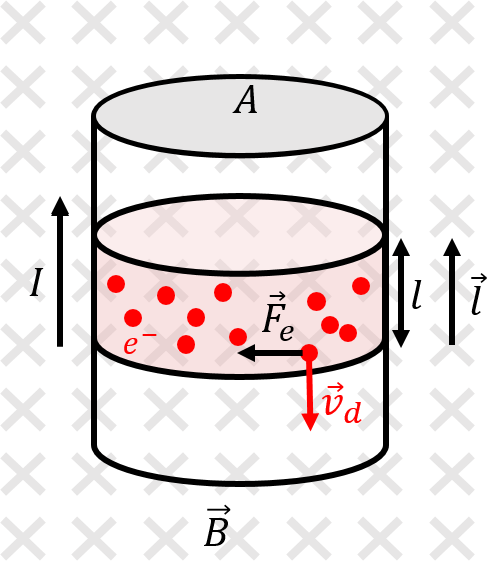
\includegraphics[width=0.3\linewidth]{files/microforce-e8a90f317eda4fec4aff9ff43bc985d4.png}
\caption[]{A section of wire carries conventional current, $I$, upwards while being immersed in a uniform magnetic field, $\vec B$, into the page. We introduce a vector, $\vec l$, to represent a section of wire of length $l$ carrying current in the direction of $\vec l$.}
\label{fig:magneticforce:microforce}
\end{figure}

A single electron (with charge $q= -e$) will experience a magnetic force, $\vec F_e$, given by:
\begin{equation}
\vec F_e = -e \vec v_d \times \vec B
\end{equation}
as illustrated in Figure~\ref{fig:magneticforce:microforce}. A section of wire of length, $l$, will contain $N=nAl$ drifting electrons, where $n$ is the density of free electrons for the wire (the number of electrons per unit volume that are available to produce a current). Thus, the magnetic force on that section of wire will be $N$ times the force on a single electron:
\begin{equation}
\vec F = N\vec F_e = nAl (-e \vec v_d \times \vec B)=-nAle \vec v_d \times \vec B
\end{equation}
Recall the microscopic model of current to relate the drift velocity to the conventional current in the wire:
\begin{equation}
I &= -nAev_d
\end{equation}
where the minus sign indicates that negative electrons flow in the opposite direction from the conventional current. We also introduce a vector, $\vec l$, with a magnitude equal to the length of the section of wire, and a direction that is parallel to the conventional current (thus anti-parallel to the electron drift velocity). The force on the section of the length, $l$, of the wire is thus given by:
\begin{equation}
\vec F = -nAle \vec v_d \times \vec B
\end{equation}
\begin{equation}
\boxed{ \vec F= I \vec l \times \vec B}
\end{equation}

\begin{framed}
\textbf{Olivia's Thoughts}\\
If you forget this formula, you can obtain it rather easily from $\vec F=q\vec v\times \vec B$. For simplicity, we assume velocity is constant, so that velocity is the displacement, $\vec l$, per unit time. We can then rewrite the formula for the force as:
\begin{equation}
\vec F&=q\vec v\times \vec B\\
&=q\frac{\vec l}{t}\times \vec B\\
&=\frac{q}{t}\vec l\times \vec B.
\end{equation}
In the last line, I have rewritten the equation to highlight the charge per unit time $q/t$, which is just the (constant) current, $I$. Using the current, the equation becomes,
\begin{equation}
\vec F=I\vec l\times \vec B,
\end{equation}
as we found previously. This is a less rigorous derivation than what we did above, but it is helpful if you just need to remind yourself of the formula.
\end{framed}

\begin{framed}
\textbf{Checkpoint}\\
\begin{figure}[!htbp]
\centering
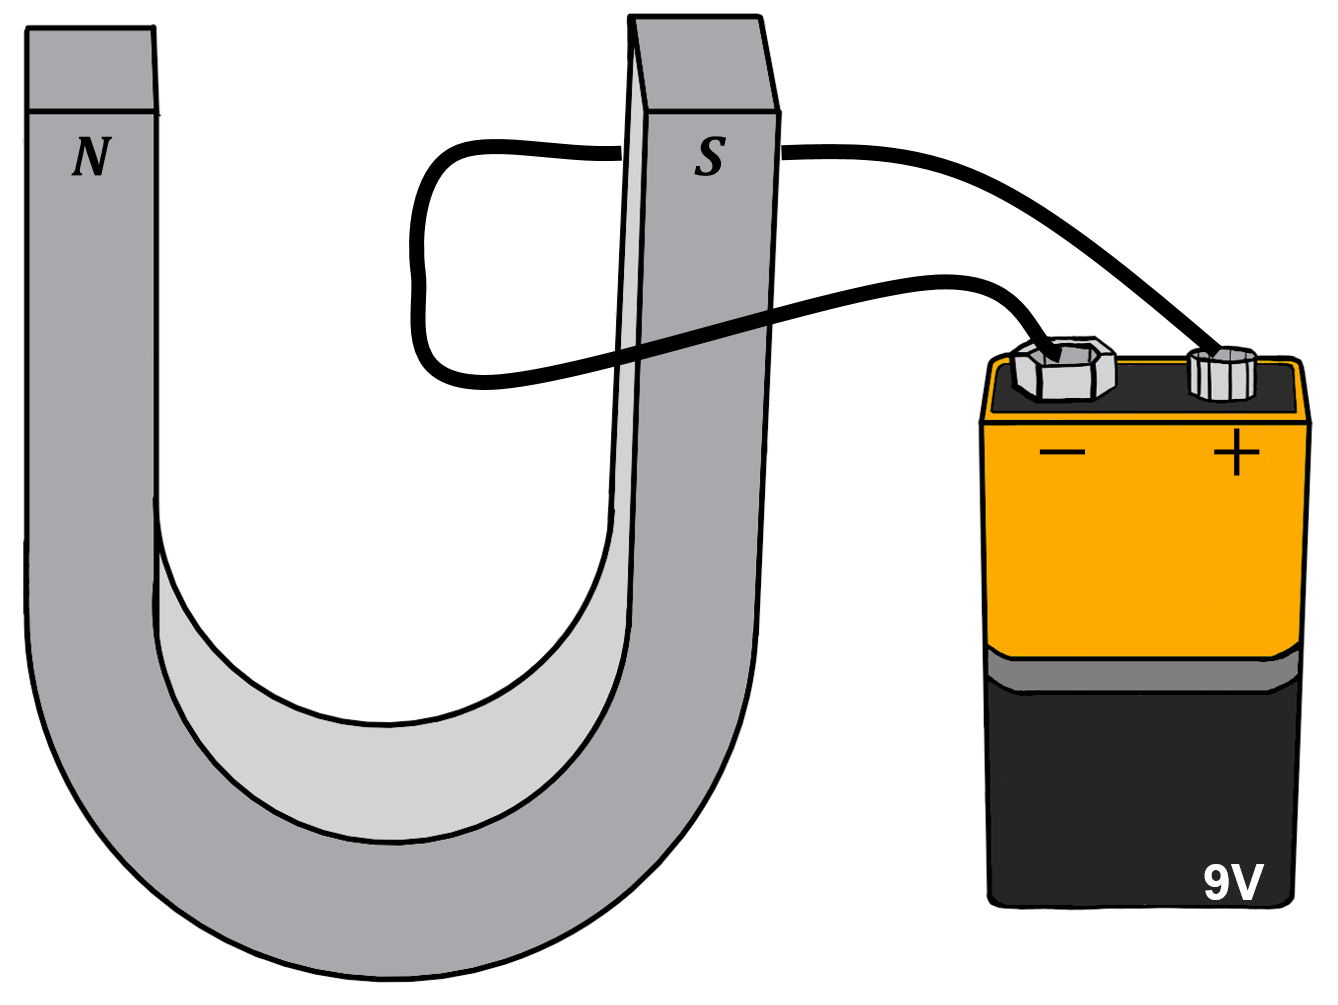
\includegraphics[width=0.35\linewidth]{files/horseshoemagnet-90d031fef6cc196c5bd44a9829c50a69.png}
\caption[]{A current carrying wire moving through a magnetic field.}
\label{fig:magneticforce:horseshoemagnet}
\end{figure}

In which direction does the magnetic force point on the current-carrying wire that is placed in the magnetic field between the poles of the horseshoe magnet shown in Figure~\ref{fig:magneticforce:horseshoemagnet}?

\begin{enumerate}
\item Up.
\item Down.
\item Into the page.
\item Out of the page.
\end{enumerate}

\begin{framed}
\textbf{Answer}\\
\begin{enumerate}
\item
\end{enumerate}
\end{framed}
\end{framed}

Note that if the wire is not straight, then we can model the wire as being made of many infinitesimally short sections (Figure~\ref{fig:magneticforce:bentwire}), of length $dl$, and sum the forces on those sections to get the total force on a section of length $L$:
\begin{equation}
\vec F = \int_0^L I d\vec l \times \vec B
\end{equation}
\begin{figure}[!htbp]
\centering
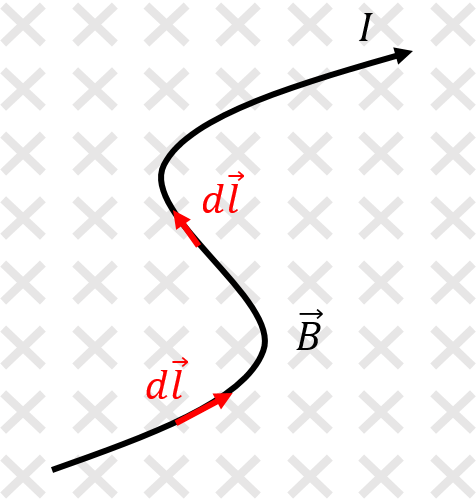
\includegraphics[width=0.3\linewidth]{files/bentwire-55e9968fb877a8a926c6dd1b897ed8e1.png}
\caption[]{The magnetic force on a curved current-carrying wire is obtained by modelling the forces exerted on infinitesimal sections of wire, each with length $d\vec l$, and summing together those forces to get the total force on the wire.}
\label{fig:magneticforce:bentwire}
\end{figure}

\begin{framed}
\textbf{Example 20.2}\\
A wire carrying current $I$ is bent so as to have a semi-circular section with radius $R$, as shown in Figure~\ref{fig:magneticforce:semicircle}. The wire is immersed in a uniform magnetic field, $\vec B$, that is perpendicular to the plane of the wire, as shown. Using the given coordinate system, what is the net force on the wire?

\begin{figure}[!htbp]
\centering
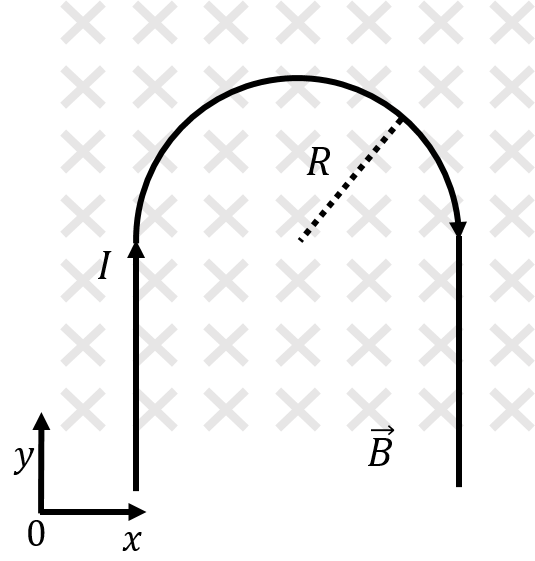
\includegraphics[width=0.4\linewidth]{files/semicircle-f5436b96732b568551593ddb5463e158.png}
\caption[]{A current-carrying wire with a semi-circular section is immersed in a uniform magnetic field.}
\label{fig:magneticforce:semicircle}
\end{figure}

\begin{framed}
\textbf{Solution}\\
We can model the wire as being made of three sections: a straight section carrying current in the positive $y$ direction, a curved section, and another straight section carrying current in the negative $y$ direction.

Consider the first straight section, carrying current in the positive $y$ direction. The force on that section of wire, by the right hand rule, will be towards the left (negative $x$ direction):
\begin{equation}
F_S &= I \vec l \times \vec B\\
&= I (l\hat y) \times (-B\hat z)\\
&= -IlB (\hat y \times \hat z)\\
&=-IlB\hat x
\end{equation}
where $l$ is the (unknown) length of that section of wire. The force exerted on the other straight section of wire will have the same magnitude, but the opposite direction (since the current, and thus the vector $\vec l$, is in the opposite direction). Thus, the forces from the two straight sections of the wire cancel, as illustrated in Figure~\ref{fig:magneticforce:semicircle_sol}.

\begin{figure}[!htbp]
\centering
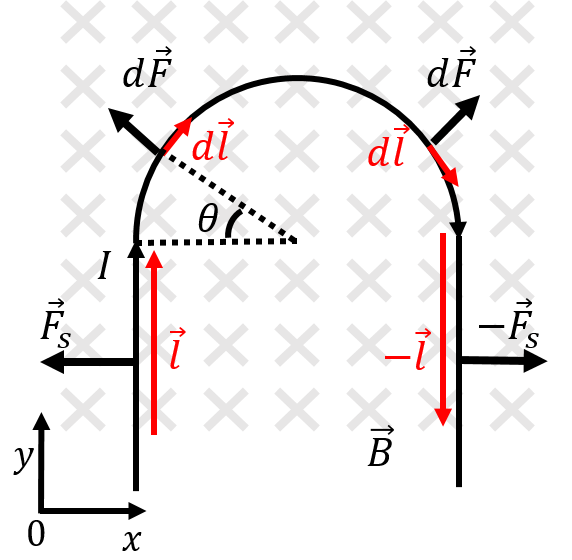
\includegraphics[width=0.4\linewidth]{files/semicircle_sol-3a4aea39b14c75d335f7088ec6b14073.png}
\caption[]{The magnetic force on different sections of wire.}
\label{fig:magneticforce:semicircle_sol}
\end{figure}

In order to calculate the force exerted on the semi-circular section, we need to add together the forces exerted on the infinitesimal sections of the wire that make up that section. Consider the magnetic force on the two infinitesimal sections illustrated in Figure~\ref{fig:magneticforce:semicircle_sol}. The $x$ components of the forces will cancel, whereas the $y$ components will add. Thus, by symmetry, we anticipate that the net force on the semi-circular section will be in the positive $y$ direction.

Consider the small force on the section of wire located at an angle, $\theta$, as illustrated in Figure~\ref{fig:magneticforce:semicircle_sol}. We can write the vector $d\vec l$ as:
\begin{equation}
d\vec l = dl(\sin\theta\hat x + \cos\theta \hat y)
\end{equation}
Thus, the infinitesimal force on that section of wire is given by:
\begin{equation}
d\vec F &= I d\vec l \times \vec B \\
&= I dl(\sin\theta\hat x + \cos\theta \hat y)\times (-B\hat z)\\
&=-IBdl (\sin\theta\hat x \times \hat z + \cos\theta \hat y \times \hat z)\\
&=-IBdl (-\sin\theta \hat y + \cos\theta\hat x) \\
&= IBdl\sin\theta \hat y - IBdL\cos\theta \hat x\\
& = dF_y\hat y + dF_x \hat x
\end{equation}
where, in the last line, we explicitly wrote out the $x$ and $y$ components of the infinitesimal force vector. In order to sum together these infinitesimal forces, it is most convenient to use the angle $\theta$ to identify each segment. $d\theta$ is related to $dl$, since $dl$ is the length of the circle subtended by the infinitesimal angle $d\theta$:
\begin{equation}
dl = Rd\theta
\end{equation}
Summing together all of the $y$ components of the infinitesimal forces:
\begin{equation}
F_y = \int dF_y = \int_0^\pi IBR\sin\theta d\theta=IBR \int_0^\pi\sin\theta d\theta=2IBR
\end{equation}
Note that the $x$ components sum to zero, as we predicted from symmetry:
\begin{equation}
F_x = \int dF_x = -\int_0^\pi IBR\cos\theta d\theta=-IBR \int_0^\pi\cos\theta d\theta=0
\end{equation}
The net force on the wire is thus given by:
\begin{equation}
\vec F = 2IBR\hat y
\end{equation}
\textbf{Discussion:} In this example we found the magnetic force on a curved section of current-carrying wire. The calculation was simplified by symmetry arguments, as we could use the right hand rule to anticipate that the force would have no component in the $x$ direction. This is because there is as much current flowing in the positive $y$ direction as there is in the negative $y$ direction, so that the corresponding forces cancel. There is however a net flow of charges in the positive $x$ direction, leading to a net force in the positive $y$ direction. As a corollary, the net magnetic force on any closed loop of current must be zero.
\end{framed}
\end{framed}

\subsubsection{The torque on a current-carrying loop}

\begin{framed}
\textbf{Review}\\
Before proceeding, you may wish to review:

\begin{itemize}
\item Section~\ref{sec:rotationaldynamics:torque} on torque.
\item Section~\ref{sec:chargesfields:electricdipole} on electric dipoles.
\end{itemize}
\end{framed}

As noted in Example~20.2, the net magnetic force on any closed loop immersed in a uniform magnetic field is zero. Consider, for example, the current-carrying rectangular loop of height $h$ and width $w$, immersed in a uniform magnetic field, $\vec B$, as illustrated in Figure~\ref{fig:magneticforce:rectangleloop} (note that the field is not perpendicular to the plane of the loop, as it was in Example~20.2).

\begin{figure}[!htbp]
\centering
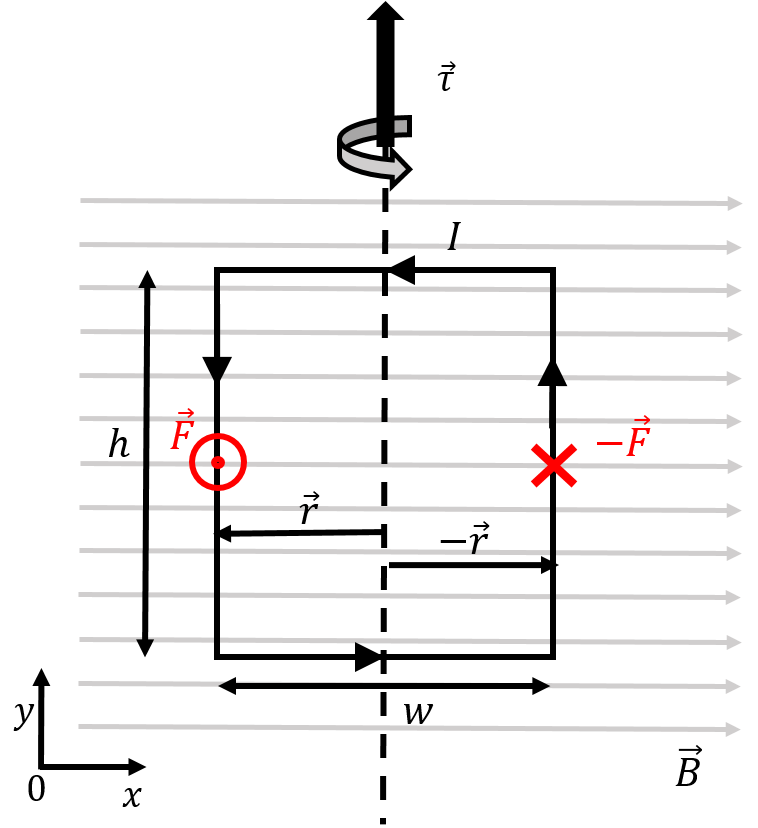
\includegraphics[width=0.4\linewidth]{files/rectangleloop-8b237152477798e6ba19d2377c451e8d.png}
\caption[]{A rectangular loop carrying counter-clockwise current in a uniform magnetic field.}
\label{fig:magneticforce:rectangleloop}
\end{figure}

The magnetic force on the two horizontal sections of the wire are zero, since the current is co-linear with the magnetic field along those sections. In the left vertical section (with current flowing downwards), the magnetic force is out of the page (positive $z$ direction), and is given by:
\begin{equation}
\vec F = IhB\hat z
\end{equation}
Similarly, the force on the right vertical section (with current flowing upwards) will have the same magnitude but the opposite direction. The net force on the loop is thus zero.

However, the net torque on the loop about its vertical axis of symmetry (shown by the vertical dashed line in the figure) is not zero. The total torque is found by summing the torques from the forces exerted on the two vertical sections of wire:
\begin{equation}
\vec \tau &= \vec r\times \vec F + (-\vec r \times - \vec F)\\
&= 2 \vec r \times F = 2 \left(-\frac{w}{2}\hat x\right) \times IhB\hat z = IBwh (-\hat x\times \hat z)\\
\therefore \vec \tau&=IBwh (\hat y)
\end{equation}
where $\vec r$ is the vector from the axis of rotation to the location where the force is exerted.

\paragraph{Magnetic dipole moment}\label{sec:MagneticForce:dipolemoment}

Describing the torque on a loop can be difficult in three dimensions, so we introduce the ``magnetic dipole moment'' to simplify the description.

If a closed loop carries a current, $I$, the magnetic dipole moment vector, $\vec \mu$, is defined such that it has a magnitude:
\begin{equation}
\mu = IA
\end{equation}
where $A$ is the area enclosed by the loop. The direction of the magnetic dipole moment vector is such that it is perpendicular to the surface defined by the loop. This leaves two possible directions, and the correct option is given by the right-hand rule for axial vectors; by curling the fingers in the direction of the current, the thumb will point in the direction of the magnetic dipole moment. This is illustrated in Figure~\ref{fig:magneticforce:momenthand}.

\begin{figure}[!htbp]
\centering
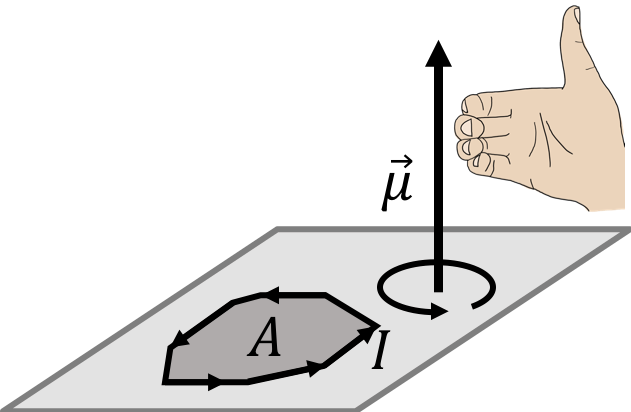
\includegraphics[width=0.4\linewidth]{files/momenthand-86ce0b6ea5974b01e75dd2e12f255f73.png}
\caption[]{The right hand rule for axial vectors is used to determine the direction of the magnetic dipole moment vector for a loop carrying current, $I$.}
\label{fig:magneticforce:momenthand}
\end{figure}

In terms of the magnetic dipole moment, the torque on a loop with magnetic dipole moment, $\vec \mu$, immersed in a magnetic field, $\vec B$, is given by:
\begin{equation}
\boxed{\vec \tau = \vec \mu \times \vec B}
\end{equation}
The magnitude of the torque is given by:
\begin{equation}
\tau =\mu B \sin\theta
\end{equation}
where $\theta$ is the angle between the magnetic dipole moment and the magnetic field vectors.

We can verify that this formula gives the correct torque for the rectangular loop in Figure~\ref{fig:magneticforce:rectangleloop} that we calculated above. The magnetic dipole moment of that loop is given by:
\begin{equation}
\vec \mu = IA \hat z = Iwh\hat z
\end{equation}
where the direction of the vector is given by the right hand rule for axial vectors (out of the page, since the current is in the counter-clockwise direction in Figure~\ref{fig:magneticforce:rectangleloop}). The torque on the loop is thus:
\begin{equation}
\vec \tau = \vec \mu \times \vec B = (Iwh\hat z) \times (B\hat x) = IBwh (\hat y)
\end{equation}
as we found previously.

The magnetic dipole moment can be used to describe a current-carrying loop in a magnetic field. That is, instead of drawing a loop carrying current, we can equivalently simply draw the associated magnetic dipole moment vector. This is useful because the magnetic dipole moment vector behaves in the same way as a bar magnet (with the tip of the arrow acting like a North pole). Indeed, a magnetic field will always create a torque that will try to align the magnetic dipole moment with the magnetic field, just as the needle of a compass experiences a torque if it is not aligned with the magnetic field of the Earth. The torque from the magnetic field is then zero when the magnetic dipole moment is parallel to the magnetic field (as the cross-product between co-linear vectors is zero).

Figure~\ref{fig:magneticforce:looptorque} shows a way to visualize a current-carrying loop in a magnetic field using its magnetic dipole moment vector, $\vec \mu$.

\begin{figure}[!htbp]
\centering
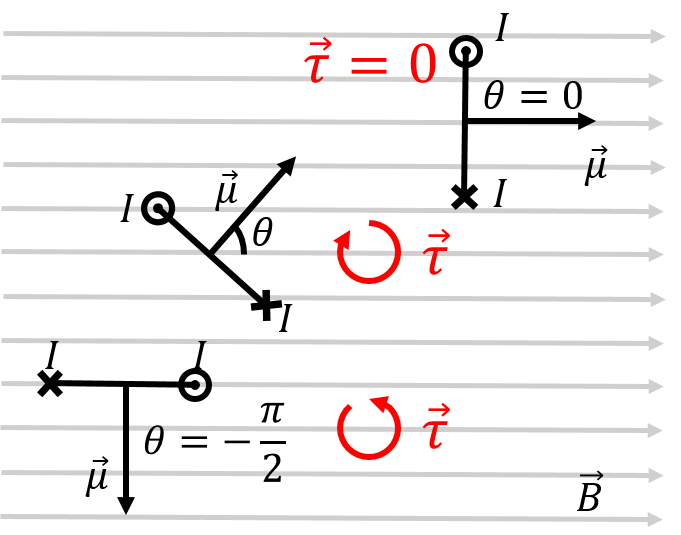
\includegraphics[width=0.4\linewidth]{files/looptorque-b927579e38704625c1187c37c60b60b6.png}
\caption[]{Three loops of current with different orientations relative to a uniform magnetic field. The loops are seen from above, and the current is shown coming in and out of the page on each loop, along with the corresponding magnetic dipole moment vector.}
\label{fig:magneticforce:looptorque}
\end{figure}

Three loops are shown (as lines), seen from above, and the direction of the current in each loop is shown as going in or out of the page. Equivalently, one can simply draw the magnetic dipole moment vector for each loop (perpendicular to the plane of the loop). For the top loop, the magnetic dipole moment is parallel to the magnetic field, so the magnetic field exerts no torque. For the middle loop, the magnetic dipole moment makes an angle $\theta$ with the magnetic field vector, so that the torque on that loop has a magnitude given by $\tau=\mu B \sin\theta$, and points into the page (clockwise rotation). The bottom loop makes an angle of $-\pi/2$ with the magnetic field, which results in a torque in the counter-clockwise direction. In all cases, the torque is such that it always tries to align the magnetic dipole moment vector with the magnetic field, just as if the magnetic dipole moment were the needle of a compass.

\begin{framed}
\textbf{Example 20.3}\\
Determine the magnetic dipole moment of the electron orbiting a hydrogen atom, if you assume that the electron is in a circular orbit with a radius of $R=0.5 \overset{\circ}{\rm A}$.

\begin{framed}
\textbf{Solution}\\
As the electron orbits around the circle, it results in a circular loop of current, $I$. The current is the rate at which charge passes through a point per unit time. If the electron orbit has a period, $T$, then the corresponding current, $I$, is given by:
\begin{equation}
I=\frac{\Delta Q}{\Delta t} = \frac{e}{T}
\end{equation}
The centripetal force on the electron is provided by the Coulomb force, $F_C$, exerted by the proton, which allows us to obtain the orbital speed, and thus the period of the orbit:
\begin{equation}
F_C &= m\frac{v^2}{R}\\
k\frac{e^2}{R^2}&= m\frac{v^2}{R}\\
\therefore v &=\sqrt{\frac{ke^2}{mR}}\\
\therefore T &= \frac{2\pi R}{v}
\end{equation}
The magnetic dipole moment is then given by:
\begin{equation}
\mu &= IA\\
&= \frac{e}{T} \pi R^2\\
& = \frac{ev}{2\pi R} \pi R^2\\
&=\frac{1}{2} evR\\
&=\frac{1}{2} \sqrt{\frac{ke^4R}{m}}\\
&=\frac{1}{2} \sqrt{\frac{(9e9 {\rm N/C^{2}\cdot m^2})(1.6e-19 {\rm C})^4(0.5 \overset{\circ}{\rm A})}{(9.1e-31 {\rm kg})}}\\
&=9\times 10^{24} {\rm A\cdot m^2}
\end{equation}
\textbf{Discussion:} In this example we calculated the orbital magnetic dipole moment of the electron in a hydrogen atom. This was a very simple model, since in reality, electrons do not orbit atoms in circular orbits, and one must use quantum mechanics to describe the motion precisely.
\end{framed}
\end{framed}

\paragraph{Potential energy for a magnetic moment in a magnetic field}

A magnetic dipole moment in a magnetic field behaves in the same way as an electric dipole in an electric field. By analogy, we can define a potential energy, $U$, for a magnetic dipole moment, $\vec \mu$, in a magnetic field, $\vec B$:
\begin{equation}
\boxed{U =-\vec \mu \cdot \vec B =- \mu B \cos\theta}
\end{equation}
where $\theta$ is the angle between the magnetic moment and the magnetic field. If a magnetic dipole is not aligned with a magnetic field and it is released, it will start to rotate (gain rotational kinetic energy) until it reaches a minimum in potential energy ($\theta = 0$). The magnetic moment would oscillate back and forth about $\theta =0$ if there are no losses. Note that the point where $\theta = \pi$, is an unstable equilibrium.

\begin{framed}
\textbf{Checkpoint}\\
When a magnetic dipole moment is parallel with a magnetic field and points in the same direction as the magnetic field, it will have...

\begin{enumerate}
\item ... its maximum torque and maximum potential energy.
\item ... its maximum torque and minimum potential energy.
\item ... its minimum torque and maximum potential energy.
\item ... its minimum torque and minimum potential energy.
\end{enumerate}

\begin{framed}
\textbf{Answer}\\
\begin{enumerate}[resume]
\item
\end{enumerate}
\end{framed}
\end{framed}

\begin{framed}
\textbf{Checkpoint}\\
When a magnetic dipole moment is placed such that the torque from the magnetic field is maximized, it will have...

\begin{enumerate}
\item ... zero potential energy.
\item ... its minimum potential energy.
\end{enumerate}

\begin{framed}
\textbf{Answer}\\
\begin{enumerate}
\item
\end{enumerate}
\end{framed}
\end{framed}

\subsubsection{The Hall Effect}

Figure~\ref{fig:magneticforce:hallV} shows a simple circuit to illustrate the Hall effect. A flat slab of metal, with width $w$, is connected to a battery, so that current flows through the slab. The slab is immersed in a uniform magnetic field, $\vec B$, that is perpendicular to the plane of the slab.

\begin{figure}[!htbp]
\centering
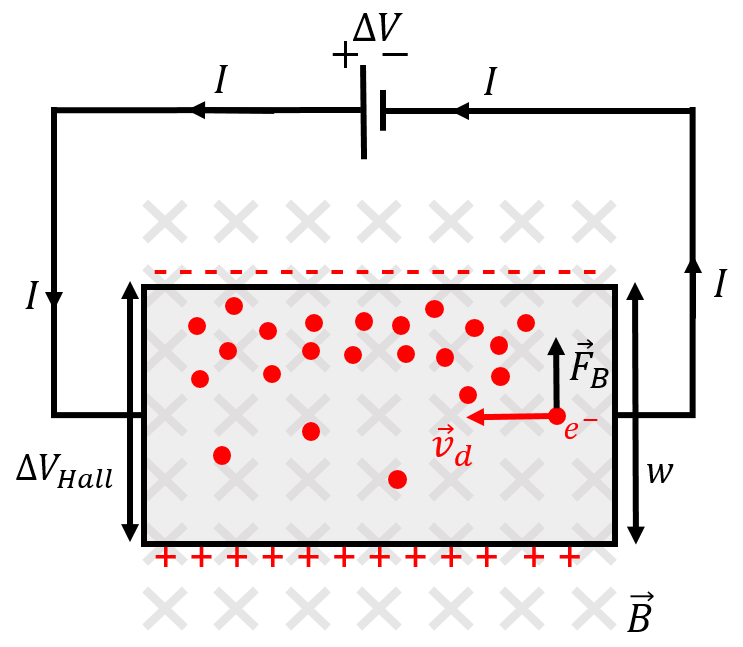
\includegraphics[width=0.4\linewidth]{files/hallV-6f069422571cd8cd2b314a481b286e52.png}
\caption[]{Illustration of the Hall effect, as electrons flow through a slab that is immersed in a magnetic field, the magnetic force pushes them to one side, creating an electric potential difference, $\Delta V_{Hall}$, transverse to the motion of the current through the slab.}
\label{fig:magneticforce:hallV}
\end{figure}

As the electrons enter the right-hand side of the slab (Figure~\ref{fig:magneticforce:hallV}) and drift towards the left, they will experience an upwards force from the magnetic field. As they move to the left through the slab, they also move upwards and ``pile up'' on that side of the slab. There will thus be an excess of negative charge on the top side of the slab, leading to an electric potential difference between the top and the bottom of the slab. This potential difference is called the ``Hall potential'', $\Delta V_{Hall}$. An equilibrium between the magnetic force and the electric force associated with the Hall potential is quickly reached, so that the Hall potential remains constant.

If we model the slab as two parallel plates, with a potential difference, $\Delta V_{Hall}$, between them, the electric field in the slab is constant and given by:
\begin{equation}
E= \frac{\Delta V_{Hall}}{w}
\end{equation}
The equilibrium condition (that the electric force on an electron is equal to the magnetic force) is given by:
\begin{equation}
F_E &= F_B\\
eE &= ev_dB\\
\frac{\Delta V_{Hall}}{w} &= v_d B\\
\therefore \Delta V_{Hall}&= v_d wB
\end{equation}
If the drift velocity of electrons is known, then the Hall effect can be used to measure the strength of the magnetic field by simply measuring the Hall voltage. This is the most common way to measure the strength of a magnetic field (and the device to do so is called a Hall probe). Conversely, if the magnetic field is known, the Hall effect can be used to characterize the drift velocity of electrons and other microscopic quantities for the material from which the Hall probe is made.

The Hall effect allows us to determine that it is negative charges that flow, and not positive charges. Indeed, consider Figure~\ref{fig:magneticforce:hallV}, but replace the electrons with positive charges flowing to the right, which is equivalent as far as analysing the circuit goes. In this case, those positive charges will be deflected upwards. Thus, if positive charges flow, the top side of the Hall probe becomes positive, whereas it becomes negative if it is negative charges that flow. By measuring the sign of the Hall potential, one can show that it is electrons that flow in an electric current.

\subsubsection{Applications}

In this section, we briefly outline a few applications of the magnetic force.

\paragraph{Velocity selector and mass spectrometer}

In Example~20.1, we described how charged particles with different charge-to-mass ratios will undergo uniform circular motion with different radii, if they all have the same speed. This principle is used in mass spectrometers, which are devices that are able to detect trace amounts of matter in a sample. For example, when your bag gets swiped with a sticky tape at a security check at the airport, that piece of sticky tape is then analysed by a mass spectrometer.

The tape is vaporized in a way to ionize the atoms on the tape. The ions are then accelerated through an electric potential difference and then pass through a region with a magnetic field. The ions typically execute half of a circular orbit before being detected, as illustrated in Figure~\ref{fig:magneticforce:massspec}. The charge-to-mass ratio of the ions is determined from the radius of their orbit. Usually, their charge is either one or two times the electron charge, allowing their mass to be determined.

\begin{figure}[!htbp]
\centering
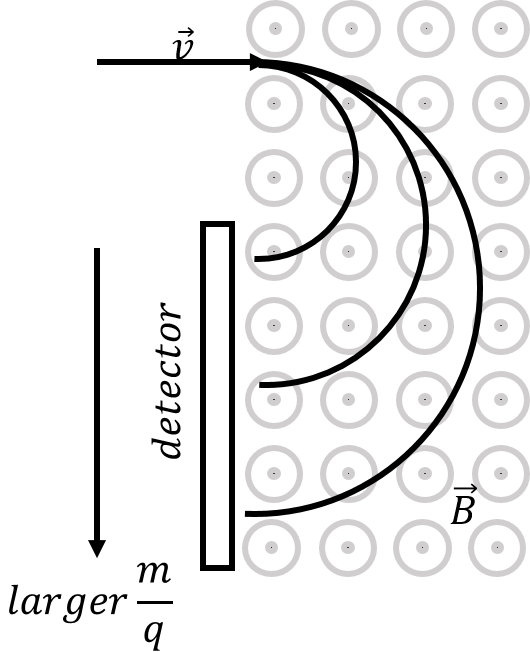
\includegraphics[width=0.4\linewidth]{files/massspec-154fd37f36c600e9f118cf7854e2640c.png}
\caption[]{Illustration of how a mass spectrometer can separate ions based on their charge-to-mass ratio. A detector is placed to measure the number of ions that appear at each radius, allowing the composition of a sample to be determined.}
\label{fig:magneticforce:massspec}
\end{figure}

In order for the mass spectrometer to function as designed, it is important that all of the charged particles enter the region of magnetic field with the same speed. A velocity selector is a device that combines perpendicular electric and magnetic fields in order to select only particles of a certain speed, regardless of their mass. The velocity selector is illustrated in Figure~\ref{fig:magneticforce:vselector}

\begin{figure}[!htbp]
\centering
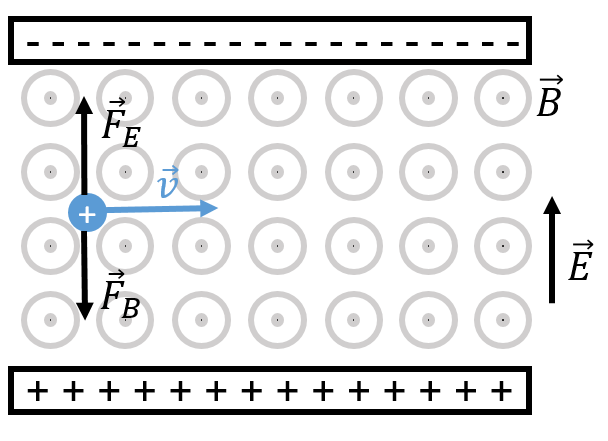
\includegraphics[width=0.4\linewidth]{files/vselector-f385c931befd350dfceb4d97c71b0e72.png}
\caption[]{Illustration of a velocity selector. Only charged particles with a specific speed can make it through without colliding with one of the plates.}
\label{fig:magneticforce:vselector}
\end{figure}

In a velocity selector, both an electric and a magnetic force are exerted. Figure~\ref{fig:magneticforce:vselector} shows a positive particle moving toward the right with speed $v$. The particle will experience an upwards electric force and a downwards magnetic force. If those two forces are equal, then the particle will move in a straight line. If, instead, one of the forces is larger than the other, the particle will be deflected and hit one of the charged plates. The condition for the two forces to be equal is given by:
\begin{equation}
F_B &= F_E\\
qvB &= qE\\
\therefore v=\frac{E}{B}
\end{equation}
Thus, the electric and magnetic fields can be tuned so that their ratio gives the desired speed. Note that the speed selector works regardless of the sign of the charge or its mass, which makes it ideal to filter the particles entering a mass spectrometer.

\paragraph{Galvanometer}

The galvanometer makes use of the magnetic force in order to measure electric current. In a galvanometer, a coil (composed of many loops) is placed in a known magnetic field. As current passes through the coil, the magnetic dipole moment of the coil increases, and the magnetic field exerts a torque on the coil. The torque from the magnetic force is balanced by the restoring torque of a torsional spring (a coil spring). A needle is attached to the coil, and the deflection of the needle, proportional to the current in the coil, is then a measure of the current through the coil. A galvanometer is illustrated in Figure~\ref{fig:magneticforce:galvanometer}.

\begin{figure}[!htbp]
\centering
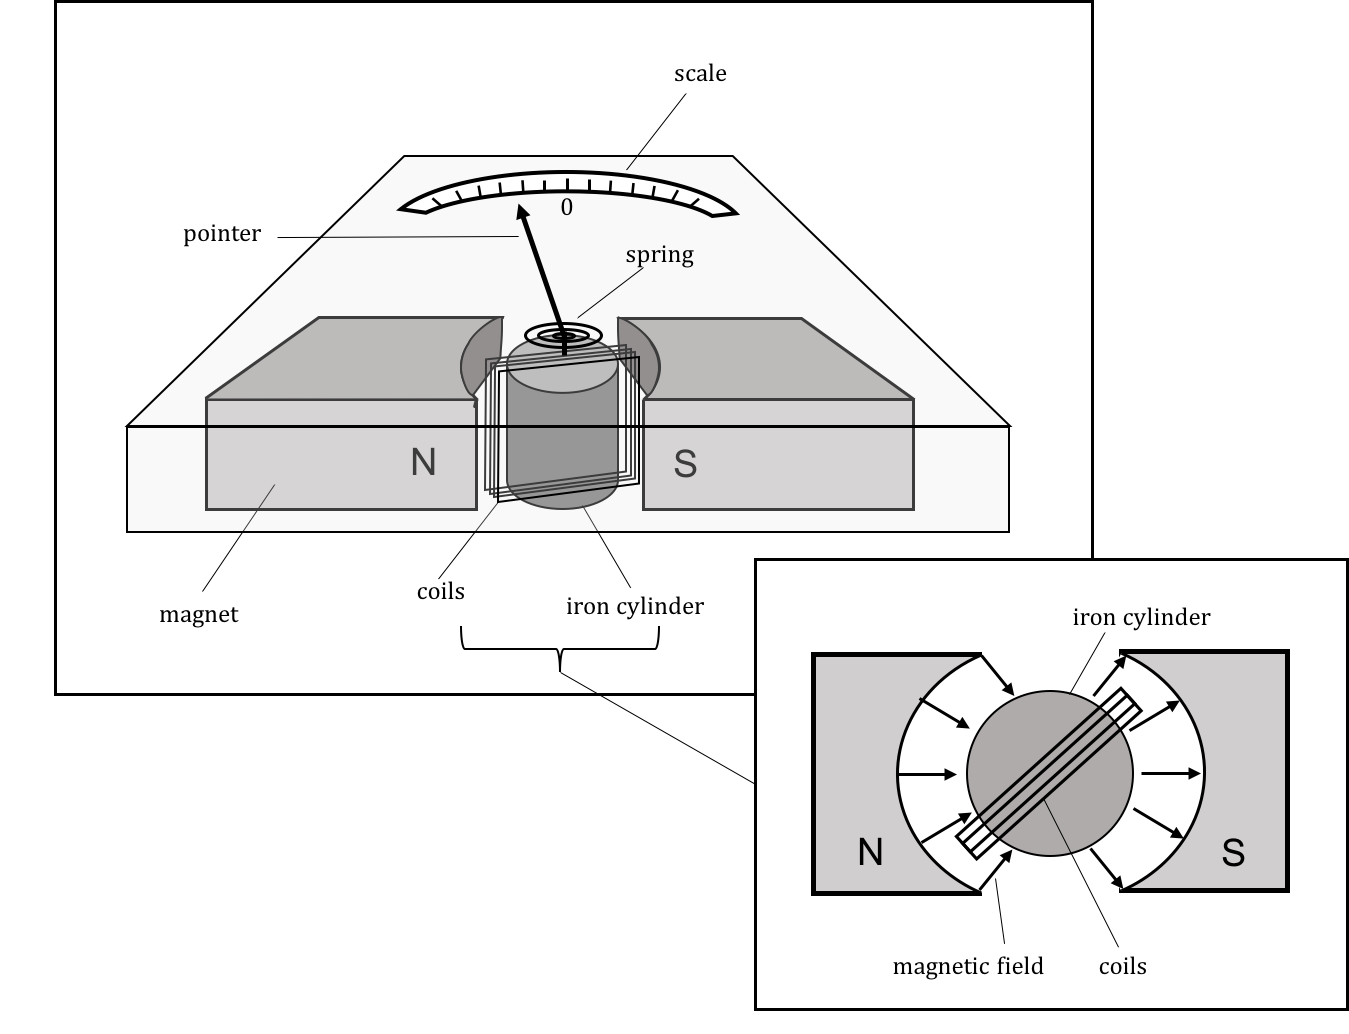
\includegraphics[width=0.7\linewidth]{files/galvanometer-b584663c2138305af4139116ae45af13.png}
\caption[]{Illustration of a galvanometer. Current passes through the coil, and the coil rotates due to the torque from a magnetic field created by a permanent magnet. The torque from the magnetic force is balanced by a torsional spring.}
\label{fig:magneticforce:galvanometer}
\end{figure}

\paragraph{Electric motor}

In an electric motor, a current-carrying coil is immersed in a fixed and uniform magnetic field. As current passes through the coil, the coil experiences a torque and rotates. Once the coil has reached a position where its magnetic dipole moment vector is parallel to the magnetic field, the direction of the current is reversed, so that the coil continues to feel a torque for another half turn, until the direction of the current is reversed again. This is illustrated in Figure~\ref{fig:magneticforce:dcmotor}.

\begin{figure}[!htbp]
\centering
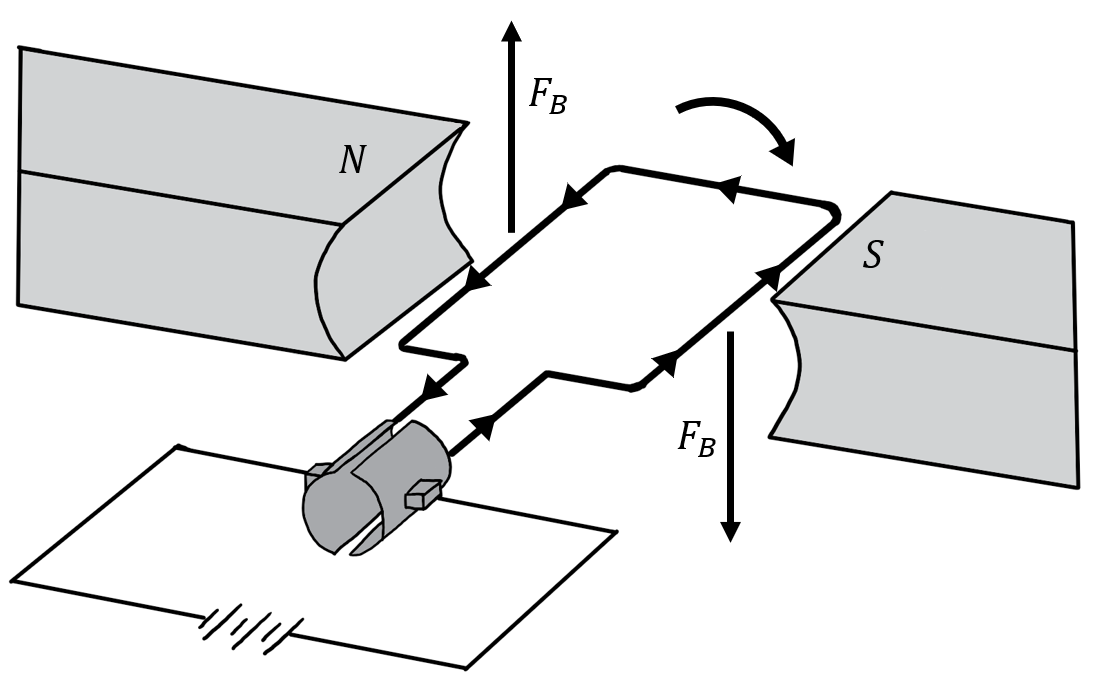
\includegraphics[width=0.65\linewidth]{files/dcmotor-719f79ce1ca8e1c208426aca4192c7e9.png}
\caption[]{Illustration of a DC electric motor. Current circulates in the coil resulting in a torque from the magnetic field. Once the coil is aligned with the magnetic field, the direction of the current in the coil is inverted, so that the coil continues to feel a torque. The current is inverted using mechanical brushes that reverse the leads on the coil every half turn.}
\label{fig:magneticforce:dcmotor}
\end{figure}

\paragraph{Cathode ray tube}

The cathode ray tube is the main component of old televisions and monitors. In those devices, a beam of electrons is accelerated by an electric potential difference. The electrons then hit a phosphorescent screen that emits light when the electrons collide with the screen. A magnetic field is used to deflect the electron beam to different parts of the screen and create the desired image, in a rapid sweeping motion, fast enough that the human eye cannot detect the sweeping motion. An example of a cathode ray tube is shown in Figure~\ref{fig:magneticforce:crt}.

\begin{figure}[!htbp]
\centering
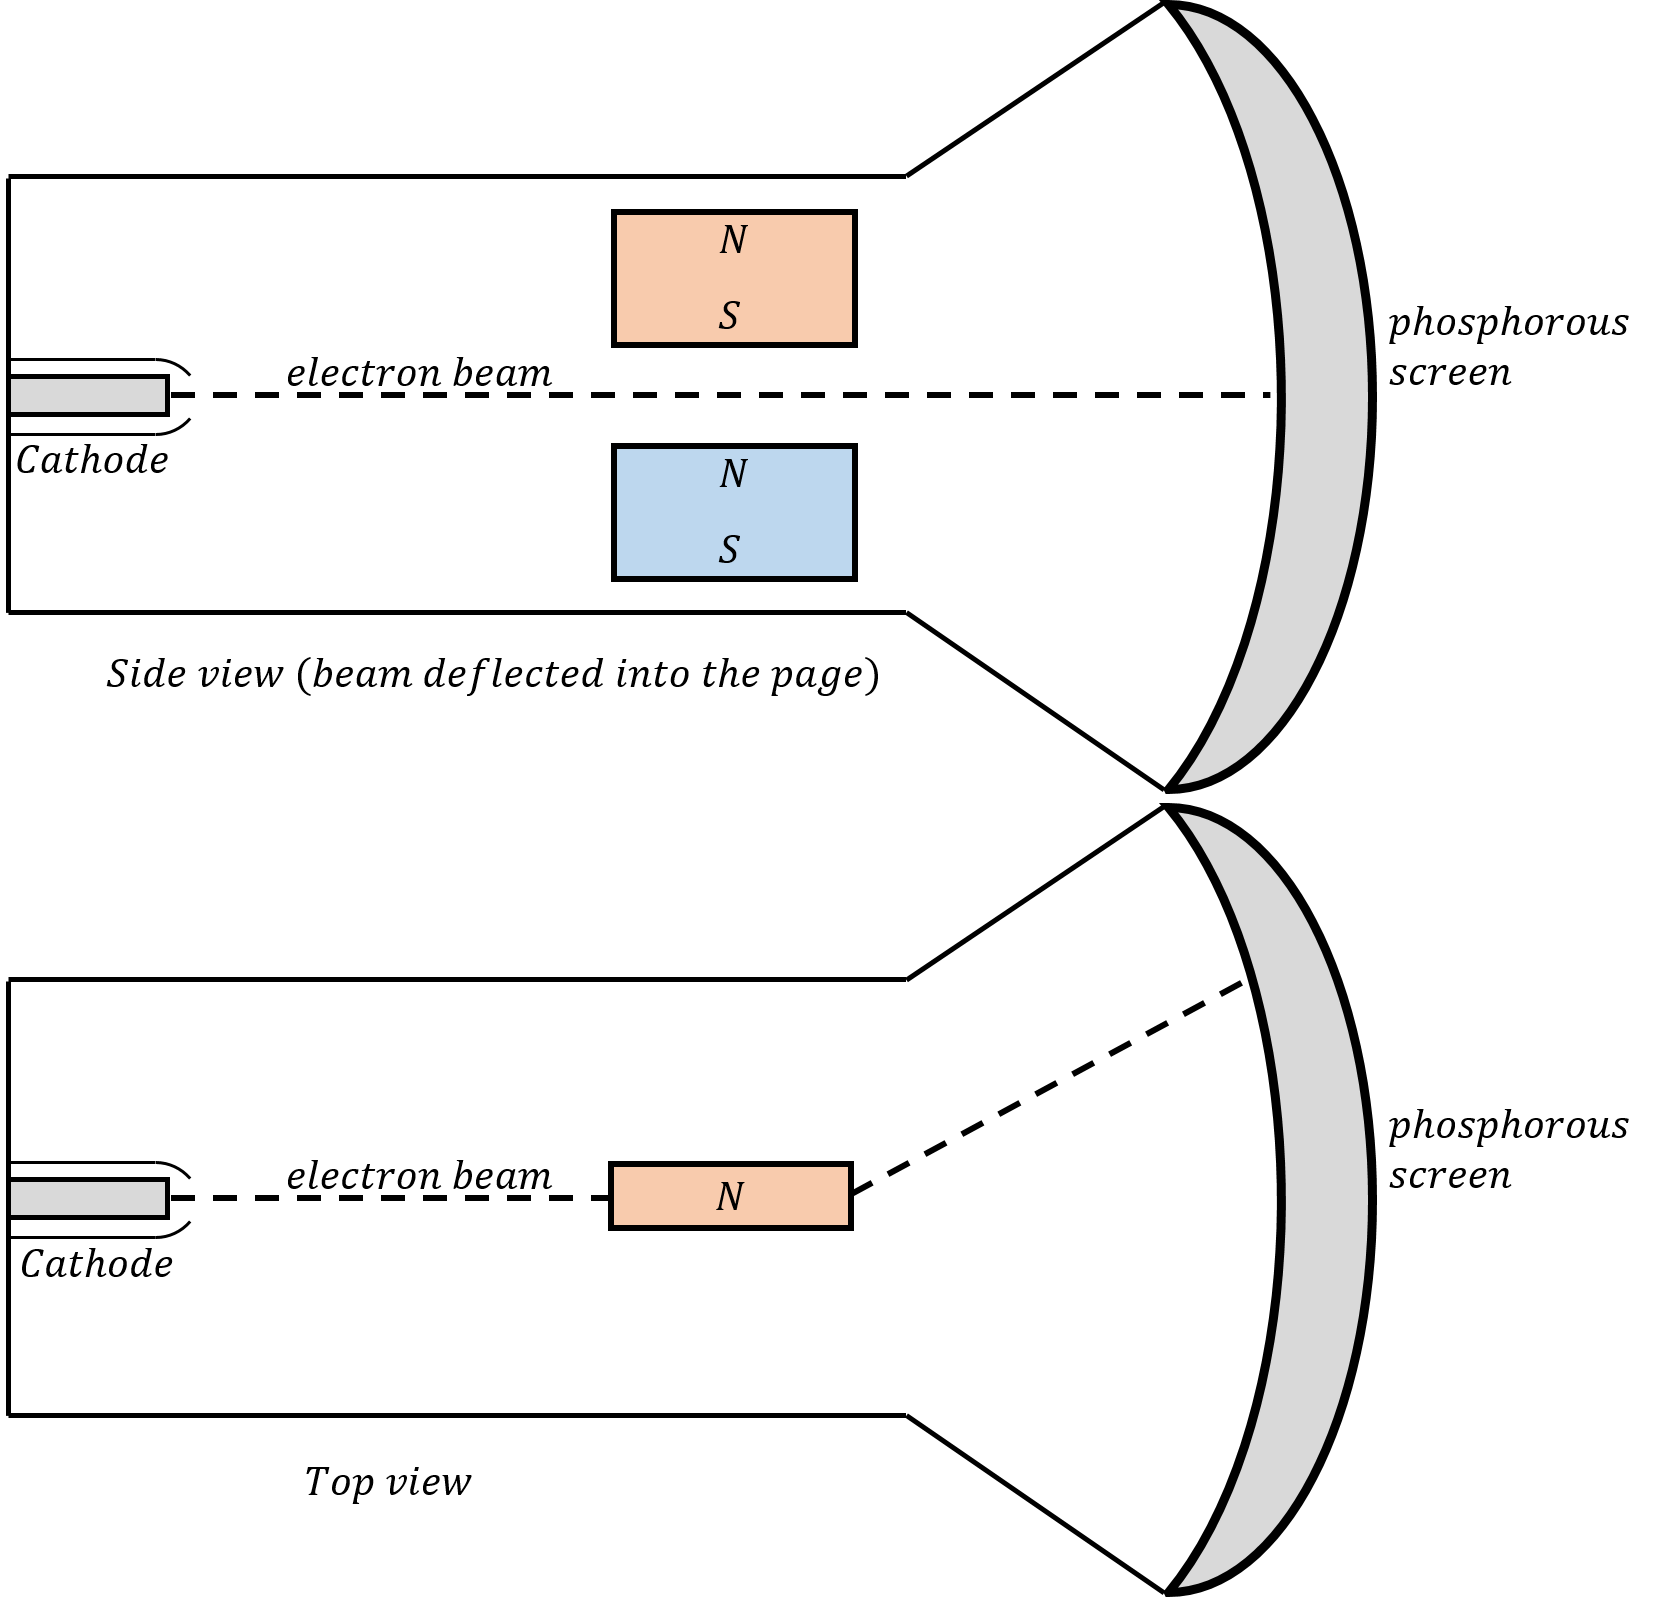
\includegraphics[width=0.6\linewidth]{files/crt-97511c9399fef59cfc4ace3b6c9ba420.png}
\caption[]{Illustration of a cathode ray tube from a side view (top) and a top view (bottom). A magnetic field is used to deflect a beam of electrons onto a screen. The perpendicular magnetic fields are used to sweep the beam rapidly across the whole screen to create an image.}
\label{fig:magneticforce:crt}
\end{figure}

\paragraph{Loudspeaker}

In a loudspeaker, a coil is immersed in a non-uniform magnetic field. The coil is attached to a membrane so that the membrane moves with the coil when a magnetic force is exerted on the coil. AC current circulates in the coil, with the same frequencies as the desired sound. The coil then moves at those frequencies and the membrane then displaces the air, creating the desired sound waves.

\begin{figure}[!htbp]
\centering
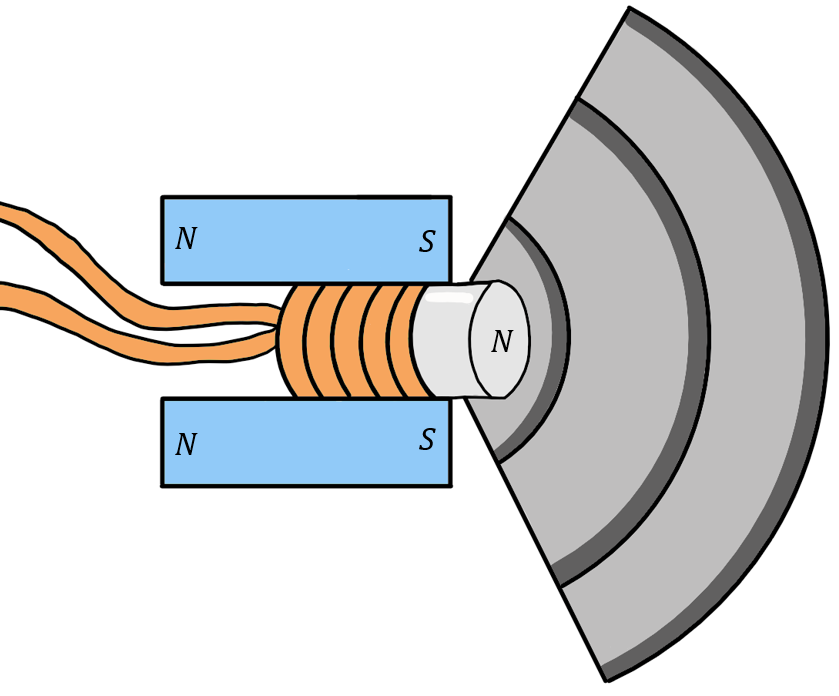
\includegraphics[width=0.6\linewidth]{files/speaker-2732a20fcc5a641b167b5f7a3c7be97e.png}
\caption[]{Illustration of a loud speaker. As current moves through the coil, the coil is pushed back and forth by the magnetic force exerted by a permanent magnet. The motion is transferred to a membrane that move the air and creates the sound wave.}
\label{fig:magneticforce:speaker}
\end{figure}

\subsubsection{Summary}

In order to describe the magnetic force, we introduced the magnetic field, $\vec B$. While there are some similarities with the electric field, the key difference in magnetism is that there are no ``magnetic charges'' (so-called monopoles), and magnets thus always have a North \textit{and} a South pole. As a result, magnetic field lines never end and must always form closed loops. The magnetic field points in the direction of the force that would be exerted on the North pole of a magnet placed at that position.

Electric charges can feel a force from a magnetic field only if they are moving relative to the frame of reference in which the magnetic field is described. If a charge, $q$, has velocity, $\vec v$, in a magnetic field, $\vec B$, it will feel a magnetic force given by:
\begin{equation}
\vec F_B =q \vec v \times \vec B
\end{equation}
The magnetic force can do no work, since it always acts in a direction perpendicular to the velocity (and thus to the displacement). The magnetic field acts in opposite directions for charges of opposite signs.

In a uniform magnetic field, a charged particle with charge, $q$, mass $m$, and velocity vector, $\vec v$, perpendicular to a magnetic field, $\vec B$, will undergo uniform circular motion, with a cyclotron radius, $R$, given by:
\begin{equation}
R &= \frac{mv}{qB}
\end{equation}

A straight wire of length, $l$, carrying current, $I$, will experience a magnetic force in a magnetic field, $\vec B$:
\begin{equation}
\vec F_B = I \vec l \times \vec B
\end{equation}
where the vector $\vec l$ points in the same direction as the current.

If the wire is curved (or the magnetic field changes direction along the wire), then we can integrate the force, $d\vec F$, exerted on each infinitesimal section of wire with length, $d\vec l$. Again, the direction of $d\vec l$ is in the same direction as the current in the wire. The infinitesimal force on an infinitesimal section of wire, is given by:
\begin{equation}
d\vec F = I d\vec l \times \vec B
\end{equation}

A closed loop of wire carrying current will experience no net force in a uniform magnetic field. However, it will experience a torque, if the loop is not ``aligned'' with the magnetic field (the torque is zero if the magnetic field is perpendicular to the plane of the loop). We define the magnetic dipole moment, $\vec \mu$ of a loop of wire carrying current, $I$, to be a vector with magnitude:
\begin{equation}
\mu = IA
\end{equation}
where $A$ is the area enclosed by the loop. The magnetic dipole moment vector is perpendicular to the plane of the loop, and points in the direction given by the right-hand rule for axial vectors applied to the current (think of the current as rotating in the loop).

The torque from a magnetic field, $\vec B$, exerted on a loop with a magnetic dipole moment, $\vec \mu$, is given by:
\begin{equation}
\vec \tau = \vec \mu \times \vec B
\end{equation}
The torque is zero when the magnetic dipole moment vector is parallel to the magnetic field vector (corresponding to the loop being ``aligned'' with the magnetic field). One can think of the magnetic dipole moment as a small bar magnet, or the needle of a compass, that always experiences a torque to align it with a magnetic field.

We can define the potential energy of a magnetic dipole moment in a magnetic field as:
\begin{equation}
U= -\vec \mu \cdot \vec B = \mu B \cos\theta
\end{equation}

The Hall effect can be observed when current flows through a slab that is immersed in a magnetic field that is perpendicular to the slab. As the electrons move longitudinally through the slab, they will also be pushed to one side by the magnetic force, resulting in an excess of negative charge on that side. An electric potential difference (the ``Hall potential'') is then established between the two sides of the slab (in the direction perpendicular to the motion of the electrons). The Hall potential is given by:
\begin{equation}
\Delta V_{Hall}&= v_d wB
\end{equation}
where $w$ is the width of the slab in the perpendicular direction, $B$ is the strength of the magnetic field, and $v_d$ is the drift velocity of electrons. The most common use of the Hall effect is to build a Hall probe to measure magnetic fields. However, Hall probes can also measure the drift velocity of electrons and other microscopic properties. The sign of the Hall potential also indicates the sign of the charges moving in the slab.

There are many applications of the magnetic force in our daily lives, including electric motors, loudspeakers, cathode ray tubes, mass spectrometers, and galvanometers.

\begin{framed}
\textbf{Important Equations}\\
\textbf{Magnetic force on a moving charge:}
\begin{equation}
\vec F_B &= q\vec v\times \vec B
\end{equation}

\textbf{Magnetic force on a current-carrying wire:}
\begin{equation}
\vec F_B = I \vec l \times \vec B
\end{equation}

\textbf{Cyclotron radius:}
\begin{equation}
R &= \frac{mv}{qB}
\end{equation}

\textbf{Magnetic dipole moment:}
\begin{equation}
\mu = IA
\end{equation}

\textbf{Torque on a magnetic dipole:}
\begin{equation}
\vec \tau &= \vec \mu \times \vec B
\end{equation}
\end{framed}

\begin{framed}
\textbf{Important Definitions}\\
\begin{itemize}
\item \textbf{Magnetic field:} A field used to model the magnetic force. SI units: ${\rm \left[{T}\right]}$. Common variable(s): $\vec B$.
\item \textbf{Magnetic dipole moment:} A property of an object which describes the torque it will experience in a magnetic field. SI units: ${\rm \left[{C\cdot m^2\cdot s^{ -1}}\right]}$. Common variable(s): $\vec \mu$.
\end{itemize}
\end{framed}

\subsubsection{Thinking about the material}

\begin{framed}
\textbf{Reflect and research}\\
\begin{itemize}
\item When was magnetism first discovered?
\item What is the origin of the word ``magnetism''?
\item What experiments support that magnetic monopoles do not exist?
\item What did J.J. Thomson measure, and how?
\item How do debit and credit cards use magnetism?
\end{itemize}
\end{framed}

\begin{framed}
\textbf{To try at home}\\
\begin{itemize}
\item Attempt to construct a compass using household materials.
\end{itemize}
\end{framed}

\begin{framed}
\textbf{To try in the lab}\\
\begin{itemize}
\item Propose an experiment to measure the magnitude of Earth's magnetic field.
\item Propose an experiment to construct a galvanometer and test its accuracy.
\end{itemize}
\end{framed}

\subsubsection{Sample problems and solutions}

\paragraph{Problems}

\begin{framed}
\textbf{Problem 20.1}\\
A cathode ray tube in a television accelerates an electron from rest using a potential difference of $\Delta V=500 {\rm V}$. Once it exits the tube, the electron must be deflected upwards by a distance $h=3 {\rm cm}$ using a uniform magnetic field, $\vec B$, before striking the phosphorescent screen, which is a distance $d= 5 {\rm cm}$ away. What direction and magnitude must the magnetic field have in order to steer the electron towards its destination?
\end{framed}

\begin{framed}
\textbf{Problem20.2}\\
A galvanometer has a square coil with a side length of $a=2.5 {\rm cm}$ and $N=70 {\rm }$ loops between two magnets which generate a radial magnetic field of $B=8 {\rm mT}$. When a current runs through the coil, it generates a torque which is opposed by a spring with a torsional spring constant of $\kappa = 1.5\times 10^{ -8} {\rm Nm~rad^{ -1}}$. If the deflection of the galvanometer's needle is $0.7 {\rm rad}$, what is the current running through the coil?
\end{framed}

\begin{framed}
\textbf{Problem 20.3}\\
Integrate the torque over a circular path, using the equation $d\vec F = Id\vec l \times \vec B$, to show that the torque exerted on a circular loop of radius, $R$, carrying current, $I$, immersed in a uniform magnetic field, $\vec B$, has a magnitude given by $\tau=\mu B$, where $\vec \mu$ is the magnetic dipole moment of the loop. You may simplify the problem by modelling the loop when its magnetic moment is perpendicular to the magnetic field.
\end{framed}

\paragraph{Solutions}

\begin{framed}
\textbf{Solution 20.1}\\
First, we determine the velocity of the electron that were accelerated over a potential difference of $\Delta V=500 {\rm V}$. Their kinetic energy is given by their charge times the potential difference::
\begin{equation}
K &= e\Delta V \\
\frac{1}{2} mv^2 &= e\Delta V\\
\therefore v &= \sqrt{\frac{2e\Delta V}{m}}= \sqrt{\frac{2(1.602e-19 {\rm C})(500 {\rm V})}{(9.109e-31 {\rm kg})}}\\
 &= 1.326e7 {\rm ms^{-1}}
\end{equation}
Now that we have the velocity, we must determine the direction of the magnetic field. We know that the electron is moving directly towards the phosphorescent screen (which we will define as $\vec x$) and the electron must be deflected directly upwards (which we will define as $\vec z$). Knowing this, we can use the right hand rule to quickly determine that the magnetic force will be acting in the $-\vec y$ direction.

In the region with a magnetic field, the electron will undergo uniform circular motion with a radius give by the cyclotron radius, $R$:
\begin{equation}
R=\frac{mv}{qB}
\end{equation}

We thus need to determine the radius of that circle for the electron to arrive that desired location on the screen. A section of the circle about which the electron moves is illustrated in Figure~\ref{fig:magneticforce:deflection}.

\begin{figure}[!htbp]
\centering
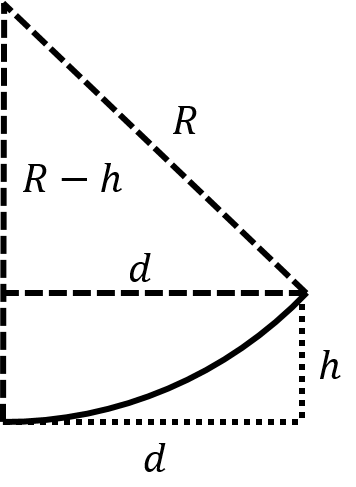
\includegraphics[width=0.2\linewidth]{files/deflection-a76b4733fa897d4bb031ad379de8324a.png}
\caption[]{Deflection of an electron moving in a uniform magnetic field.}
\label{fig:magneticforce:deflection}
\end{figure}

From geometry and Pythagoras' Theorem, we have:
\begin{equation}
R^2 &= (R-h)^2+d^2\\
R^2 &= R^2-2Rh+h^2+d^2\\
\therefore R &= \frac{h^2+d^2}{2h}=\frac{(3 {\rm cm})^2+(5 {\rm cm})^2}{2(3 {\rm cm})}=5.67 {\rm cm}
\end{equation}
The strength of the magnetic field is then given by:
\begin{equation}
B&=\frac{mv}{qR}=\frac{(9.11e-31 {\rm kg})(1.326e7 {\rm ms^{-1}})}{(1.6e-19 {\rm C})(0.0567 {\rm m})}=0.00133 {\rm T}
\end{equation}
\end{framed}

\begin{framed}
\textbf{Solution 20.2}\\
First, we will determine the magnetic dipole moment of the square coil:
\begin{equation}
\mu &= NIA\\
\mu &=NIa^2
\end{equation}
Now that we have the magnetic dipole moment, we can calculate the torque on the square coil that is produced by the magnetic field. Note that, in a galvanometer, the magnetic field is configured such that it is radial and always perpendicular to the magnetic dipole moment of the coil:
\begin{equation}
\tau_B &= \mu B sin(90 {\rm \degree})= NIa^2B\\
\end{equation}
The deflection, $\theta$, for a given current will occur when the torque produced by the wire is equal to the torque produced by the spring. The torque produced by the spring is given by:
\begin{equation}
\tau_s =\kappa \theta
\end{equation}
where $\theta$ is measured in radians. The above equation is the rotational equivalent of Hooke's Law. Equating the torque from the spring and from the magnetic field, we can determine the current:
\begin{equation}
\tau_B&=\tau_S\\
NIa^2B &= \kappa \theta\\
I &= \frac{\kappa \theta}{Na^2B} = \frac{(1.5e-8 {\rm Nm(rad)^{-1}}) (0.7 {\rm rad})}{70(0.025 {\rm m})^2(8e-3 {\rm T})}\\
&= 30 {\rm \mu A}
\end{equation}
\end{framed}

\begin{framed}
\textbf{Solution 20.3}\\
Figure~\ref{fig:magneticforce:proof1} illustrates a loop of radius, $R$, carrying current, $I$. The loop is in the $x -z$ plane, and there is a magnetic field, $\vec B$, in the negative $x$ direction. By setting the loop up this way, it is easier to visualize some of the three-dimensional aspects.

\begin{figure}[!htbp]
\centering
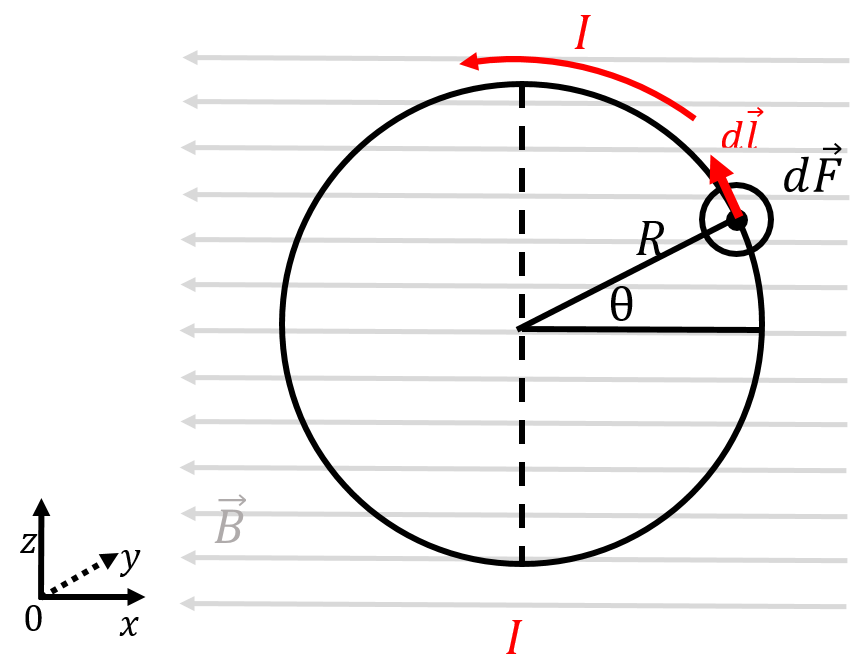
\includegraphics[width=0.5\linewidth]{files/proof1-8111f1e51bf6dd8310876d5f97bc88a5.png}
\caption[]{A current-carrying loop in a magnetic field.}
\label{fig:magneticforce:proof1}
\end{figure}

Consider an infinitesimal section of the loop, with length, $dl$, located on the loop at a position labelled by the angle, $\theta$, as illustrated. The vector, $d\vec l$, is given by:
\begin{equation}
d\vec l  = dl (-\sin\theta \hat x + \cos\theta \hat z)
\end{equation}
The magnetic force on that element of the loop is given by:
\begin{equation}
d\vec F &=Id\vec l \times \vec B\\
&=Idl(-\sin\theta \hat x + \cos\theta \hat z) \times (-B\hat x)\\
&=-IBdl\cos\theta (\hat z \times \hat x)\\
&=-IBdl\cos\theta\hat y
\end{equation}
and the force on that element of wire is out of the page (negative $y$ direction), as illustrated. That infinitesimal force will create an infinitesimal torque:
\begin{equation}
d\vec \tau = \vec r \times d\vec F
\end{equation}
where $\vec r$ is the vector from the axis of rotation (through the centre of the loop, parallel to the $z$ axis) to the point where the force is exerted. The length of the vector, $\vec r$, is simply $r=R\cos\theta$, and the force is perpendicular to the vector $\vec r$. Thus, the torque on the infinitesimal element is given by:
\begin{equation}
d\vec \tau &= \vec r \times d\vec F\\
&= (R\cos\theta \hat x)\times (-IBdl\cos\theta\hat y)\\
&=-IBR\cos^2\theta dl (\hat x \times \hat y)\\
&=-IBR\cos^2\theta dl \hat z
\end{equation}
and the torque on that infinitesimal element is in the negative $z$ direction, as anticipated from the direction of the force. Note that had we considered the loop to be oriented such that the magnetic field is not in the plane of the loop, the vector $\vec r$ in the torque would have a component in the $y$ direction.

We can sum the torques on each element of the loop, from $\theta = 0$ to $\theta=2\pi$. We can express the length, $dl$, using the infinitesimal angle, $d\theta$, that subtends the arc of length, $dl$, on the circle of radius, $R$:
\begin{equation}
dl = Rd\theta
\end{equation}

The net torque is then given by:
\begin{equation}
\vec \tau &= \int d\vec \tau\\
&=\int -IBR\cos^2\theta dl \hat z\\
&= (-IBR^2\hat z)\int_0^{2\pi} \cos^2\theta d\theta\\
&=(-IBR^2\hat z)\pi
\end{equation}
The magnetic moment of the loop is:
\begin{equation}
\mu = IA = I\pi R^2
\end{equation}
so that the torque is indeed given by $\tau = \mu B$. If we had rotated the loop so that the vector, $\vec r$, had a $y$ component, then we would have found the general formula with a cross-product.
\end{framed}